\documentclass[twocolumn,letterpaper,10pt]{article}
\usepackage{graphicx,amsmath}
\usepackage{epsf}
\usepackage[round]{natbib}
\usepackage{txfonts}
\usepackage{upgreek}
\usepackage{rotating}
\usepackage{epstopdf}
\usepackage{abstract}
\usepackage{hyperref}
\usepackage{geometry}
\geometry{margin = 0.75in}

\def \um {$\mu m$}

\title{Monte Carlo Constraint of Luminosity Evolution and Redshift of Far-Infrared Galaxy Surveys}
\author{Noah Kurinsky\\*
  \small Tufts University '14\\*
  \small Department of Physics and Astronomy}
\date{\small \today}

\begin{document}
\twocolumn[
  \maketitle
  \begin{onecolabstract}
    \centering
    This work presents a new software tool for characterizing the properties of an observational survey of galactic populations by the use of the multidimensional spectral color space over which the survey extends to fit both model and redshift distributions to the dataset. We detail in this paper the creation of this tool as well as the methodology behind it, including the assumptions made for this early version. We discuss the testing of the program, for which two surveys taken by BLAST and Herschel's SPIRE instruments were used. The software is still in early stages of development, and we discuss the additional features we plan to add, as well as the goal of being able to fully fit all characteristics of a given population. Our hope for this tool is that it can be used by the greater scientific community to improve quality and efficiency of analysis of new surveys, whether it be used to produce publishable work or guide researchers in the right direction when conducting their own analyses.
  \end{onecolabstract}
  \vspace{1cm}
]

\section{Introduction}
In the field of observational astrophysics, a great deal of time is put into characterizing various properties of surveys of galactic populations both large and small. The vast majority of these efforts focus on an analysis specific to the survey, instrumentation, and source type being studied, and each requires new computer code and months of work to produce a publishable result. The necessity of such a time commitment makes maximizing the scientific yield of such analyses a top priority. Recent attempts have been made to characterize the properties of galaxy populations by using very general spectral features (e.g. spectral color) to fit complex evolutionary models \citep[e.g. redshift-luminosity evolution, as in ][]{marsden11}. A discussion of such methods, as well as their successes and failures, can also be found in the previous reference.

We extend the ideas presented in \citet{marsden11} from one spectral color to two; whereas they attempt to fit their model using the single 60-100 $\mu$m color, we instead employ a two color model, using three spectral bands, to create a two-dimensional diagnostic spectral color density plot of an observed population. We then employ a library of multi-parameter galactic spectral energy distribution (SED) models to try to reproduce the observed trend, exploring the parameter space to constrain the redshift distribution and parameter distributions. Future versions of this program will ultimately attempt to constrain the luminosity-redshift evolution as well. 

Our novel approach allows us to characterize the sample under examination as well as highlight the successes and failure of the SED template and the luminosity function form used by the fitting procedure. In addition, a large emphasis has been put on ensuring that the fitting program is highly generalizable; the model and luminosity function are stored in external files, and thus the templates desired by the user can be specified at runtime. The program is not band or instrument specific, and the user can specify the exact survey characteristics (such as magnitude limits and statistical noise levels) to achieve the best fit possible. Such considerations allow us to address the need for reusable code, with the intent being that the analysis of data sets of this nature can be done much quicker, and result in a larger, richer science yield.

The above is a very general description of the product we detail in this paper. We begin by discussing the assumptions made by the current form of the fitting procedure, such as luminosity functional form as well as the form of the redshift and model distributions. We then discuss the mathematical methods employed to randomize the simulation, perform the fitting, and generate the fitting statistic. We then present the results of testing the program with two far-infrared data samples of the GOODS-North field obtained by BLAST \citep{BLAST} and the Spitzer FLS field obtained by the HerMES survey \citep{HerMES}, using Herschel's SPIRE instrument \citep{Herschel,SPIRE}. These data sets measure identical bands, but differ in sensitivity, sample size, sky coverage, and other minor respects. We finally lay out the improvements that we plan to implement in the near future, and our eventual goals pertaining to public release and long-term usability for the project. 

\section{Simulating Galactic Populations}

To produce a simulated galaxy population suitable for comparison to an observed population (given the analyses described later in this paper), three flux densities corresponding to three distinct bands of observation need to be produced, in numbers which reduce statistical error to an experimentally acceptable level. The models employed must be able to reproduce characteristics of a wide range of galaxies, thus a set of models must be chosen that can generally describe any galaxy. In the far-infrared regime of the electromagnetic spectrum, the vast majority of radiation from galaxies is dust-reprocessed thermal radiation, and thus the emissions from these galaxies can be characterized by a blackbody, or more accurately, a modified blackbody (see Section \ref{sec:SED}). Choosing a model derived from physical formulae, as opposed to an empirical model, allows our eventual fits to speak more to the physical characteristics of the galaxy population, which in turn allows us to eventually infer star-formation rates as well as some other basic properties simply from the combination of temperature and luminosity.

Following the above reasoning, the first step in the simulation process is to generate a template of spectral energy distributions (SEDs) of the galaxies, from which flux densities can be pulled and to which parameter distributions can be ascribed. At first glance, it would seem as though such a library alone would be adequate for the simulation purposes, however observational surveys aren't perfect data products, and thus additional corrections must be made for factors such as statistical noise characteristic of the detector in use as well as the magnitude limit of the sample. In order to correct for these and other factors, it is necessary to adopt a luminosity function, with the added ability to randomly produce luminosities for sources in accordance with their likelihood as prescribed by the function. Additionally, a luminosity distance calculator is necessary, to convert luminosities into flux densities that can be used to normalize a given SED, such that noise can be added in a realistic manner to the template. The functional form of these and other components of the simulation, as well as details of their implementation, are described later in this section.

To be able to test the accuracy of the model against observation, a diagnostic needs to be chosen which can capture as many aspects of the sample as possible. Single fluxes have little meaning, as they vary with luminosity and distance, however, the trend over the entire simulated regime is luminosity independent, and provides a means by which to identify different sub-groups of similar sources. We choose to use the spectral color (defined as $S_\nu\propto\nu^\alpha$) to characterize each source, and produce a two-dimensional histogram of the entire population from these colors to describe the cumulative properties of the sample. The construction of this histogram and the method of comparison are described later in this section.

Even though the following sections describe specific implementations of the various aspects of the fitting program, it is important to note that many of these specific forms are only those adopted for early testing of the fitting and modeling methods. The program has been designed and implemented to work with arbitrary models, and none of the specific details discussed below are actually present in the code, but are read in from files and are fully changeable. The luminosity function may, in the future, operate in a similar way. The overall design of the program is to strive for as few specific assumptions as possible. With this consideration in mind, we move on to discuss the specific assumptions made for the early version of this program.

\subsection{SED Library}\label{sec:SED}
The SED library employed for the first version of this tool consists of a set of modified black-bodies, as described earlier, which have the functional form $S_\nu(T,\beta)=B_\nu(T)\nu^\beta$, where $B_\nu(T)$ is the Planck function, $T$ is temperature in Kelvin, and $\nu$ is frequency. This effectively adds a variable power law component to the normal blackbody, which better approximates the thermal spectra of galaxies. It also gives the model a second variable parameter aside from temperature to allow for more robust fitting. 

Ideally, the program would calculate flux densities source by source, using a continuous parameters distribution to produce the eventual simulation. Since we designed the fitting program to be generalizable to any model template, this was not practical. We instead designed the program to read in a library of pre-calculated models. The library we generated has models for $\beta = 1.0,1.1,...,2.0$ and $T=10,20,...,100$, and can be seen in Figure \ref{slib}. The program generates a model space with finer resolution than the models provided by performing spline interpolations between models, so that the number of models provided has a smaller effect on the quality of the fits than would otherwise be present. This is discussed further in Section \ref{class:models}.

In order to assess the breadth of our models in relation to the spectral color space which will be used for fitting, we also made a diagnostic of the entire range of colors reproducible by the models for redshifts in the range $0<z<10$. This can be seen in Figure \ref{slib_color}. 

\subsection{Luminosity Function}

As discussed earlier, adopting a luminosity is important to simulate the effects of noise on a sample, as well as determine detectability of sources at various bands by normalizing their SEDs at a specific band. For this version of the program we employ an IRAS-type luminosity function from \citet{negrelloIP}:
$$
\frac{dN}{dV dlogL}(L|L^*_0,\Phi^*_0,\alpha,\beta,z) = \Phi^*(z)*\left[{\left(\frac{L}{L^*(z)}\right)}^{\alpha}+\left(\frac{L}{L^*(z)}\right)^{\beta}\right]^{-1}
$$
where $\Phi^*$ and $L^*$ are evolved with redshift as described in \citet{Caputi07}:
$$
\Phi^*(z) = \Phi^*_0(1+z)^p \quad
L^*(z) = L^*_0(1+z)^q
$$
The default values for $\alpha$, $\beta$, $\Phi^*_0$, and $L^*_0$ for 350 $\mu$m were taken from \citet{negrelloIP}, and the default values for p and q were taken from \citet{Caputi07} for redshift evolution out to $z\approx2$. These values only serve as defaults, and can be altered via the interactive interface, as will be discussed below.

\subsection{Cosmology}

In order to convert luminosity and redshift into a flux, as well as determine the detectability of a source given the magnitude limit of a sample, the program needed to be able to compute luminosity distance, and thus needed to be able to adopt some sort of cosmology. We decided to assume a flat universe ($\Omega_k=0$), however all other cosmological parameters are left free, so that future users can adjust them as more accurate measurements are made. Our one assumption allows for the code to be faster and more efficient, and as it is commonly believed that our universe has no curvature, it should not affect the long-term value of this program.

Luminosity distance is computed by the standard formula:
$$
d_L(z)=\frac{(1+z)c}{H_0}\int\limits_0^z\frac{dz'}{\sqrt{(1+z')^3\Omega_M+\Omega_\Lambda}}
$$
The default parameters are taken to be $H_0=73,\Omega_M=0.282,\Omega_\Lambda=0.728$, following the accepted default parameters in the IDL function {\sc{lumdist}}\footnote{http://idlastro.gsfc.nasa.gov/ftp/pro/astro/lumdist.pro} (so that the earlier IDL and C++ versions of the simulator are compatible, for testing purposes).

\subsection{Redshift and Model Distributions}

The randomized redshift and model numbers for each simulated source are produced in accordance with four different types of distributions: fixed, flat, Gaussian, and bimodal distributions, the last of which is implemented as the sum of two separate Gaussian distributions. The bimodal distribution is used only for redshift; for all other parameters, only the first three are applicable. 

For the redshift distribution, there are five free parameters, including mean and standard deviation for each Gaussian component as well as the ratio between their respective amplitudes. To implement the distribution with the chosen parameters, one Gaussian distribution is created with a fixed number of elements, while the other contains a number of elements equal to the fixed number times the variable ratio. The fixed amplitude is set to 1000 elements as a default, but can be modified via the interactive interface. The initial redshift range is set to $0<z<10$, to allow for the program to remain relevant for even the most distant surveys, however this too is modifiable by the interactive interface.

In the current version of the fitting program, the model parameters are not fit to observation but are fixed for each round of fitting, and can be modified interactively by the user. The user can choose to fix a parameter at a certain value, or generate a distribution with custom parameters. The range can be specified as well, to control the width of a fixed distribution or tightly bind a Gaussian distribution to within a strict range. Future versions will allow the distributions to be fixed or fitted, as will be discussed later in Section \ref{fdirs}.

\subsection{Correcting for Survey Properties}

In addition to simulating the theoretical SEDs produced by galaxies, a thorough fit of model to observation must take into account certain properties of the survey being analyzed. In the current version of the fitting program, random Gaussian noise representative of the average flux error is added independently to each simulated band after normalization by the luminosity function to simulate error due to unforeseen factors. In addition, the magnitude limit is taken into consideration, and sources whose flux in any band falls below the detection threshold of the instrumentation are excluded from all analyses, although the number of ``undetectable'' sources produced by various parameter combinations is recorded, so that in the future it may be used somehow to improve the quality of the fit. 

For the tests discussed in Section \ref{example}, the noise level was the experimentally found mean of the flux errors provided with the survey data, calculated separately for each band.

\section{Fitting Methodology}

The simulated and observed galactic populations are compared on the basis of their spectral color distributions, as discussed in the introduction. In order to produce a statistic indicative of goodness of fit, a diagnostic plot which can characterize an entire population based on the spectral colors of the sources is needed, in order to produce a space within which the statistic can be run. For our fitting program, we employ a two-dimensional color histogram, of which each axis is a distinct spectral color. This is discussed in further detail in Section \ref{color_hist}. 

The fitting statistic used to compare observation and simulation is a $\chi^2$ statistic, computed as described in Section \ref{chisq}. The fitting is performed by systematically varying the parameters of the various distributions in an attempt to minimize the chi-square error. For the current version of the fitting program, this is a somewhat involved process, as the model parameters are currently fixed and must be altered by the user to find the parameter distributions which produce the best fit. This process will be described in more detail as an example of the fitting is described in Section \ref{example}.

\subsection{Two-Dimensional Spectral Color Histogram}\label{color_hist}

As with all fitting programs, one of the most important choices made in the design process is choosing the way in which to compile the data such that a fitting statistic can be run on it. Most programs tend towards one dimensional data representations, as these are much easier to handle. Due to the nature of our models and of sources in this particular regime of the electromagnetic spectrum, we decided on a two-dimensional color density metric. This data representation allows us to clearly identify multiple populations where present, as well as trends at both sides of the range of interest.

The diagnostic produced from the simulated data is a two dimensional histogram, with the 250\um/500\um\ color as the x axis and the 350\um/500\um\ color as the y axis. An example of this diagnostic for a real dataset can be seen in Figure \ref{fig:hist1}. There are in fact three unique color pairs that can be produced from fluxes in three distinct bands. This combination was chosen because the 500\um\ flux has a larger statistical error than the other two bands. This combination ensures that sources with largely erroneous 500\um\ fluxes will still exhibit the same general trend, but lie either lower or higher on the trend than they should be. This is not important for fitting purposes, as we add in simulated noise at comparable levels to that present in observation. It does allow for better identification of potential multiple populations by eye within a given sample and minimizes the visual noise obscuration such that overall trends are minimally disturbed.

\subsection{Chi-Square Testing}\label{chisq}

The major hurdle to working with higher dimensional metrics like this is the over abundance of zero values. Higher dimensional spaces tend to become largely empty as data sets become smaller, thus making the traditional goodness of fit methods harder to implement, as many behave poorly at small values and are undefined at 0. To help counteract this problem, we employ the binsize selection method outline in \citet{binsize}, where the ideal bin size for a sample of size $N$ with standard deviation $\sigma$ is: 
$$
\Delta \alpha=\frac{3.49\sigma}{\sqrt[3]{N}}$$
 This formula was experimentally found by \citet{binsize} to best balance the need to minimize whitespace and statistical error while maintaining as much resolution as possible.

The goodness of fit statistic we employ is the popular $\chi^2$ statistic, although a few minor alterations needed to be made to the general formula to obtain a statistic useful for our particular diagnostic, as well as to eliminate the "0" problem which plagues the traditional formula. To begin with, we assign the histogram bins standard Poisson errors ($\sigma_i=\sqrt{N_i}$). Starting from the generalized chi-square formula:
$$
\chi^2=\sum\limits_{i=1}^n \frac{(O_i-E_i)^2}{\sigma_i^2}
$$
we get our fitting statistic by setting bin error to 
$$
\sigma_i=\sqrt{\sigma_{E_i}^2+\sigma_{O_i}^2}=\sqrt{E_i+O_i}
$$ 
The chi-square error is defined so long as one of the two diagnostics has a non-zero value. For zero values, the results are in agreement, so the formula is overridden and that particular bin is assigned a $\chi^2$ value of zero. The resulting piecewise $\chi^2$ formula then becomes:
$$
\chi^2=
\begin{cases}
\sum\limits_{i=1}^n \frac{(O_i-E_i)^2}{E_i+O_i}, & O_i > 0 \text{ or } E_i > 0 \\
0, & E_i=O_i=0
\end{cases}
$$
This approach ensures that for any given comparison, there exists a $\chi^2$ value, and gives more weight to areas of higher density, as they have lower comparable error to those bins with only a few sources.

\subsection{Multidimensional Minimization}
The fitting method used in the current version of the program is a simple minimizer, which attempts to find the parameters corresponding to the lowest chi-square statistic. This is normally achieved by employing the first and second derivatives of a given function to find local and global extrema, however due to the non-linear, somewhat discontinuous nature of the relationship between parameters and chi-square values, this is impossible for the program in its current state. Instead, an algorithm which employs small guesses in an attempt to move to a location of better fit (lower error) is employed, using a best guess as a starting point. 

Though this minimization works well in some cases, there are a few concerning caveats of this approach:
\begin{enumerate}  \itemsep0pt \parskip0pt \parsep0pt
\item There is no way to restrict the minimizer to a limited parameter space
\item This approach can only find local minima and will exit when the first minimum is found, as it has no way of sampling the entire space during minimization
\item Due in part to point two, the ability of the minimizer to find the best result is highly dependent on the initial guess for the parameter values
\item The minimization technique requires random guesses to sample the space, and due to the fact that the space is highly irregular and may contain tens of minima, given starting parameters will often result in very different results.
\end{enumerate}
In order to reduce the effects of these issues, we find the best fit of ten minimization attempts. This will also allow us to estimate uncertainties for our parameter values in future versions of the program if we continue to use this method (which seems highly unlikely at the present). The minimization technique is one of the many features of this program which we intend to improve upon, as will be discussed in Section \ref{fdirs}.

\section{Implementation}

The software tool consists of two distinct parts, created to work in tandem to read in data, perform a fitting pass, and display the best fit model. The top-level interface and graphing utilities were programmed in IDL, a high-level interactive programming language uniquely suited for astronomical applications, creation of interactive widgets, and graphing. The actual fitting was performed by a program written in C++, a lower-level language better suited to implementing computationally complex tasks which require the ability to enhance programming efficiency.

\subsection{C++ Executable}

As described above, the C++ portion of the program performs the fitting of the data. It takes two Flexible Image Transport System (FITS)\footnote{A file format commonly used to store and transport astronomical data, more compact and efficient than text files} files as input, one for observation and the other for models and parameters. The program produces a third file as output, containing the best fit parameter distributions as well as the model, observation, and comparison histograms. The majority of the input and output operations are performed by the CCFits library\footnote{CCFITs \citep{CCFITS} is an open source C++ library designed to facilitate the development of programs utilizing FITS files in C++. It is largely an extension of the older CFITSIO \citep{CFITSIO} package, originally designed for the C programming language. The CFITSIO package provides a more object-oriented, higher level interface for the old-library's routines.} procedures. Our program mainly provided C++ wrappers where necessary to organize data into structures compatible with CCFits routines or to decode data extracted from files. 

For the more complicated mathematical operations, such as interpolation, random number generation, integration, or minimization, various GNU Scientific Library (GSL)\footnote{The GNU Scientific Library \citep[GSL, ][]{GSL} is a compilation of C++ procedures for use in scientific programs, designed to provide well documented, well tested, and highly efficient methods for performing mathematical operations as well as carrying out higher level analyses.} functions are employed to maximize efficiency and take advantage of the superb algorithms provided with the package. The specific functions used for each of these four operations by various classes are described below:

\paragraph{Random Number Generation}

All functions which generate random numbers are based off of the procedures and algorithms outlined in Chapter 18 of \citet{GSL}. These procedures instantiate a generator from a chosen algorithm and provide the interface by which to get uniformly distributed random variates. For this program, the default algorithm ({\sc gsl\_rng\_mt19937}) is employed. Documentation and further description of this algorithm can be found in the above citation. The random number generator is seeded with a random variate produced by the C++ function {\sc{srand}}, which is in turn seeded with the current time and date. It should be noted that this seeding procedure is temporary and will be revised in future versions of this program. 

A method for generating Gaussian random number distributions as well as a method to generate random numbers with an arbitrary probability distribution are also used, taken from Chapter 20 of \citet{GSL}.  C++ wrapper functions were written for these GSL procedures so that custom ranges, means, and standard deviations could be applied when applicable, and so that large arrays of random deviates could be generated ahead of simulation.

\paragraph{Numerical Integration}

Numerical integration is performed while calculating luminosity distance, and is combuted by the GSL QNG non-adaptive Gauss-Kronrod integration function and related procedures, outlined in Chapter 17 of \citet{GSL}.

\paragraph{Interpolation}

Interpolation is necessary for many aspects of the simulation and is used heavily by multiple classes. Both linear ({\sc{gsl\_interp\_linear}}) and cubic spline ({\sc{gsl\_interp\_cspline}}) interpolation methods are used in the program, and are described in more detail in Chapter 27 of \citet{GSL}. The library provides methods that store the values for interpolation as well as those which require them to be passed in for every evaluation. These were both used, the prior when many interpolations were to be done and memory to be conserved, the latter when speed was desired and only a few interpolations would be performed on any given data set. Similar consideration led to the choice between linear and cubic spline interpolation.

\paragraph{Multidimensional Minimization}

The current method for parameter fitting employs a multidimensional minimization function from the GSL library, described in Chapter 36 of \citet{GSL}. This function, like the other GSL functions, is highly parametrized, and allows for various algorithms to be employed. The default algorithm for minimization without the use of derivatives ({\sc gsl\_multimin\_fminimizer\_nmsimplex2}) is used in the current version of the program. The variable parameters are stored in a GSL vector container, while a reference to the simulator and the fixed parameters are passed to the minimizer via a custom structure. More algorithmic and structural details can be found in the above citation.

\subsubsection{Classes and Other Methods}
Each distinct part of the simulation is given its own class and dedicated methods, both in good practice and to further the modular, generalized nature of the program. The classes are arranged in a hierarchy to maximize efficiency and allow for proper object oriented programming convention. 

The ``simulation'' class manages instances of ``distributions'' classes, which store and manipulate the model parameter and redshift distributions. The ``simulator'' class manages the ``simulation'' class, ``model library'' class, and the ``histogram'' and ``observation'' classes. It also communicates with the ``luminosity function" class. The simulator class returns $\chi^2$ values for the simulation obtained from the parameter values it is given. The top level ``main'' procedure manages the luminosity function and simulator classes, and performs the minimization of the model. It also calls the various functions responsible for saving output when a minimum is found. Specific implementation details for each class are discussed below.

\paragraph{Distributions Class}
The distributions class manages both the model parameter and redshift distributions, and provides an interface for specifying whether a fixed, flat, or Gaussian distribution is desired. In addition, any of these can also be added to the existing distribution, if it has already been initialized. This class makes heavy use of the random number generation methods described earlier in this section.

\paragraph{Model Library Class}\label{class:models}
The model library class reads the provided model templates from a FITS file and stores them in a one dimensional array, indexed in relation to its parameter values. The library compensates for the finite number of models by allowing for cubic spline interpolation between them for any band and redshift combination, provided that the model ids, bands, and redshifts are all within allowable ranges. The three model flux values used for interpolation are produced by finding three models that bracket the arbitrary model desired and extracting fluxes corresponding the band requested, red-shifted appropriately. Bands are extracted from individual models by spline interpolation as well, thus providing the illusion from outside the class that any arbitrary parameter/band combination is contained within. The finer the resolution provided in the model template fed to the program, however, the lower the errors due to interpolation will be. 

\paragraph{Luminosity Distance Calculator}
The luminosity distance calculator is a member function of the Luminosity Function Class, however it can be called by any function to get the distance for any redshift. To improve the efficiency of this function, all distances for the given redshift range are pre-computed to a resolution of $z=0.01$, and the resulting values are then used to initialize a cubic spline interpolator. Subsequent calls to the luminosity distance method thus perform an interpolation, which is much faster and more efficient than integrating to that redshift at every function call.

\paragraph{Luminosity Function Class}
The Luminosity Function Class is responsible for providing the normalization factor for simulated SEDs. It first initializes luminosity functions evolved to each redshift in the allowable range in increments of $z=0.1$, and then instantiates a random number generator for each redshift, using the corresponding luminosity function as a probability distribution. The luminosity functions are set so that the lower luminosity range stops at the flux corresponding to the detection limit for the given redshift. When a flux density for a given redshift is requested, the function generates a random luminosity, and computes the k-corrected flux for that redshift.

\paragraph{Observation Class}
The observation class reads the matched fluxes and survey properties from a FITS file and instantiates "source" structures for each set of fluxes. These source structures compute the appropriate spectral colors and store them such that the observation class can return two color arrays to a higher function when requested.

\paragraph{Simulation Class}
This class contains the distribution classes and a reference to the model library class, and is responsible for extracting the models corresponding to the various parameter values and producing arrays of "source" structures representing a simulated survey. It returns arrays of colors in much the same way as the observation class, and is functionally equivalent in outside appearance to it. The simulation class also gets passed a reference to the luminosity function class, which allows it to normalize source SEDs and add observational noise during simulation. It checks that each source would be observed by a survey with the given properties and flags any source which should be excluded from later analysis on grounds of being undetectable (this only happens if multiple attempts to normalize the SED all result in undetectable sources).

\paragraph{Histogram Library Class}
The histogram library class creates the histograms for observed and simulated color arrays, and compares them, computing and returning the chi-square goodness of fit statistic. This class uses the observation arrays to calculate optimal bin size and histogram range, and then computes the model histogram based on these values. The class is designed such that the observation values only need to initialized once, regardless of the number of simulations performed, and each time the model is re-initialized, the comparison histogram and chi-square error are updated. This class also contains methods for saving the histograms to a FITS file.

\paragraph{Simulator Class}
The simulator class essentially controls, instantiates, and manages all classes except for the luminosity class. It is responsible for taking the input from the minimizer and running the simulation, and then returning the chi-square statistic. It is also responsible for creating the save file and calling the various save functions for each member class when requested. The design of this class allows for the main program to consist only of a parameter fitting procedure, allowing for different fitting procedures to all rely on one class to produce fitting statistics.

\paragraph{Main Program}

The main program instantiates both the simulator and luminosity function classes, as well as the initial fitting parameters. It runs the minimization procedure and keeps track of the lowest chi-square error from all runs, telling the simulator to save whenever a minimum chi-square is achieved. It is also responsible for all console output and user interaction, where applicable. A sample of the output produced by the main program can be seen in Figure \ref{disp:fit}.

\subsubsection{Optimization and Efficiency Considerations}

Much thought was put into optimizing the program, as initial versions were very sluggish. C++ Standard Template Library containers were widely used in place of dynamic memory when possible, and static variables were used for functions with local variables which were called often. In addition, costly read/write operations were kept to a minimum, and references were passed in place of values where possible. Despite these and other considerations, the program has an average run-time of about 30 seconds, down from 2-3 minutes, however this is expected to change as methods are altered and components added.

\subsection{IDL Interactive Widget and Plotting}

The IDL widget consists of two stages, a pre-fitting and post-fitting stage. The pre-fitting stage (shown in Figure \ref{disp:init}) reads in the matched fluxes in three separate bands from an observational survey of the user's choice (saved as an IDL save file), and provides an interface by which the user can specify the parameters of each bandpass for the survey. It also allows the user to specify the parameters used for luminosity distance calculation as well as the luminosity function. The IDL code passes all of these data to the C++ fitting code by mean of FITS files.

The post-fitting stage (shown in Figure \ref{disp:res}) reads the output from the C++ fitting code and generates a set of diagnostic plots, including differential number counts for each observed band, the output luminosity function, the output redshift distribution, and the output model parameter distributions. It also displays the color-color density plots as well as their comparison. All of these diagnostics are provided as a supplement to the goodness-of-fit statistic, to double check the result by eye based on secondary metrics.

\section{Testing and Initial Results}\label{example}
During all stages of development, two sample surveys were used to test the functionality of the fitting program. The first sample was the smaller, less sensitive survey done by the Balloon Borne Large Aperture Submillimeter Telescope taken from \citet{Devlin09} of the GOODS-North field. The second sample was of the Spitzter First Look Survey (FLS) field taken from the HerMES survey \citep{HerMES}, conducted using the Herschel Space Telescope's SPIRE detectors \citep{Herschel,SPIRE}. The tests performed thus far were purely qualitative, and as of yet there are no specific results to present, however initial testing shows that the program functions are expected thus far. An example of the output produced by one of the better fitting runs can be seen in Figure \ref{disp:res}. This specific fit was performed on the HerMES data. While the general trend is well reproduced, much improvement remains to be made, as the agreement is still quite poor compared to the chi-square levels we are hoping the fitting program will be able to achieve. Future changes and enhancements, discussed in the next section, aim to improve this agreement.

\section{Future Directions}\label{fdirs}

The program in its current state is only the beginning of a larger effort to produce a reusable, highly adaptable IDL widget that can easily characterize samples obtained by multiple instruments across various bands fit with supplied models. Going forward, there are a few main areas where we expect to improve upon the program as it exist today:
\begin{itemize} \itemsep0pt \parskip0pt \parsep0pt
\item The program will be able to fit all aspects of the model, including luminosity function and model parameters, and the user will be able to specify whether any parameters or portions of the redshift distribution should be kept constant.
\item We plan to use a much improved fitting technique, such as a Markov Chain Monte Carlo, which will be capable of a)being restricted to a specific domain and b)sampling the entire space to find a global minimum, as opposed to a local minimum. Such an approach also allows for accurate estimation of parameter uncertainties and can help illuminate if and where there are degeneracies between parameters.
\item We plan to provide a wide range of built in model libraries, and update the interface to be very model-specific, so that parameter settings can be specified in terms of the actual values as opposed to library indices. It may be possible, in future version of the program, to code model functions in C++ and eliminate the need for excessive interpolation and approximation.
\item Future versions of the code will allow for selection of instrument specific bands, which will include bandpass information. This will allow us to do bandpass corrections and will simplify the analysis process, as flux and confusion limits can be optional arguments, with defaults pre-coded. We may still leave options open for users to specify custom band parameters.
\item To enhance the capabilities and provide secondary fitting methods, we plan to utilize differential counts to help fit models, as these are very well measured for many regions of the sky and provide an excellent way to check that other aspects of the simulation line up with expectation. The more addition fitting statistics we can use, the less degeneracy and ambiguity there will be in our fits.
\item More types of statistical distributions will be added in conjunction with the flat, fixed, and Gaussian forms currently used by the program.
\end{itemize}

The longterm goal for this project is to provide a tool to the astronomical community to use for many years to come. The progress made thus far is encouraging, however this is an ongoing project and one that was never intended to be completed in a few short months. We hope eventually for this work to become my senior thesis, and for the product of that thesis to be the first publicly released version of this program, however we also anticipate further work on this project beyond that point, as more complicated surveys are published and there is a need to add more detailed features to our analysis.

\bibliographystyle{plainnat}
\bibliography{writeup}

\begin{figure*}
  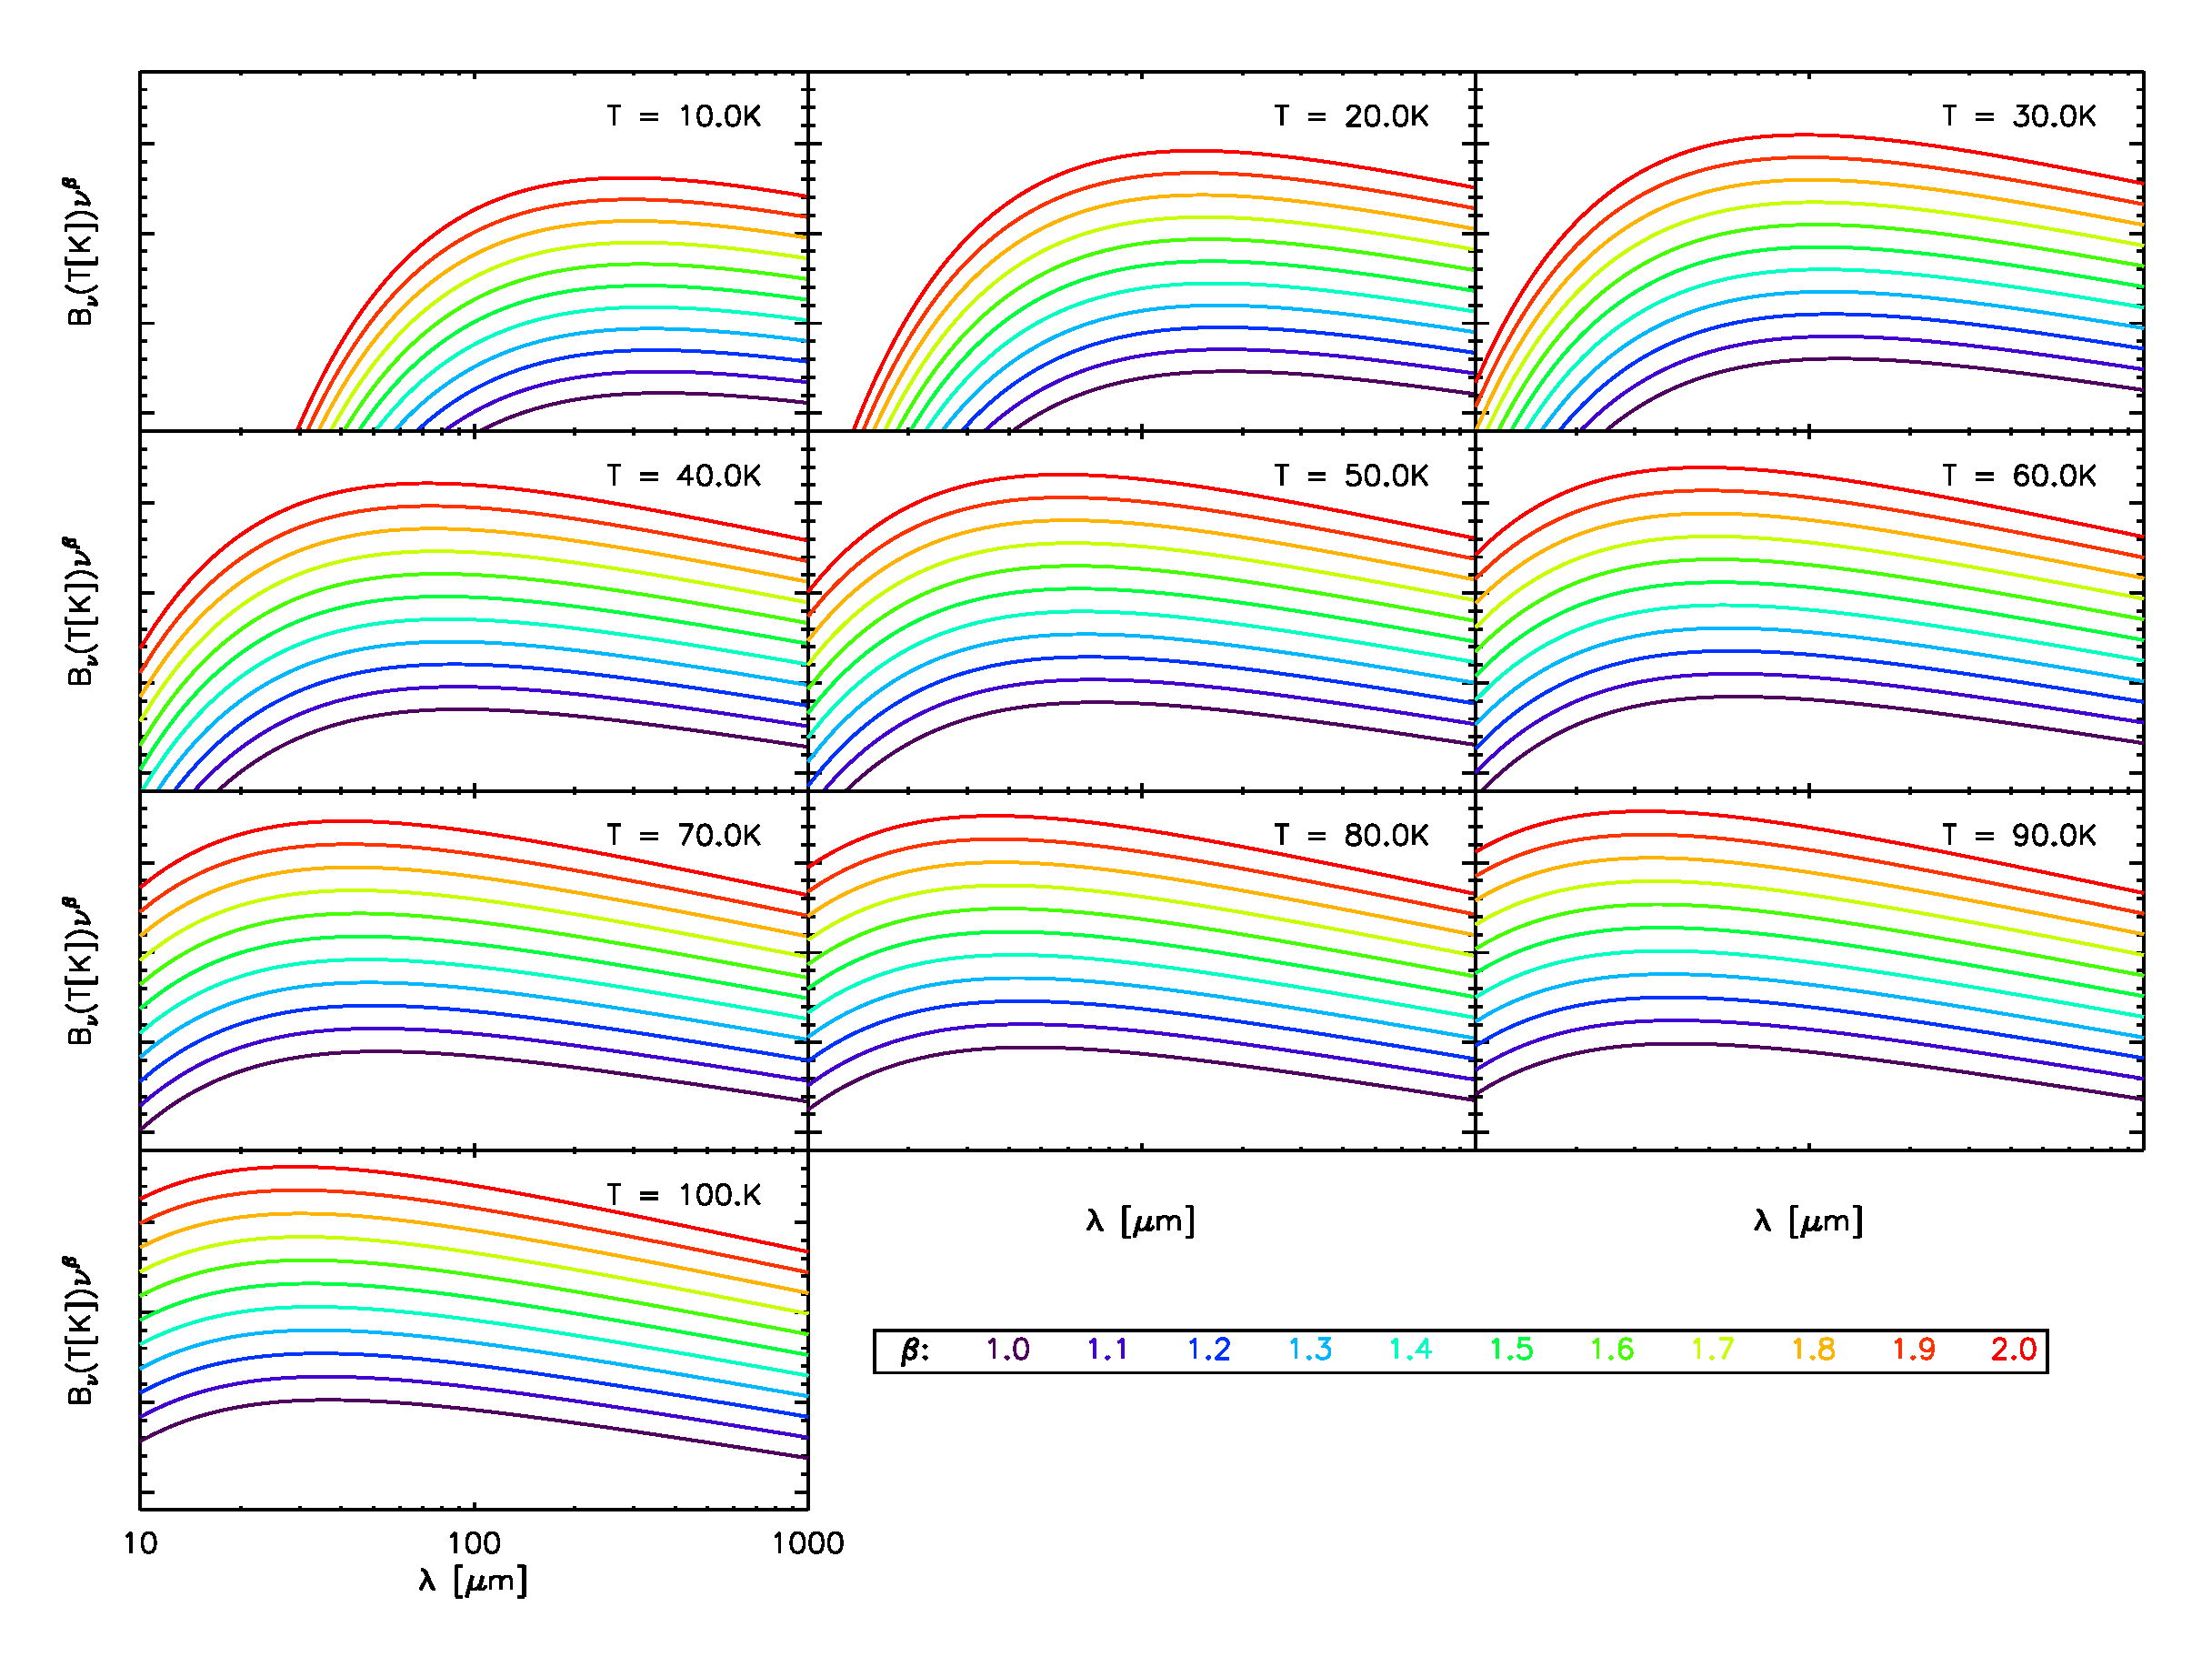
\includegraphics[width=\textwidth,trim=0.25in 0.25in 0.25in 0.25in,clip=true]{template.eps}
  \caption{SED Library consisting of modified blackbodies, of the form $S_\nu(T,\beta)=B_\nu(T)\nu^\beta$, where $B_\nu(T)$ is the Planck function, $T$ is temperature in Kelvins, and $\nu$ is frequency.  The library has models for $\beta = 1.0,1.1,...,2.0$ and $T=10,20,...,100$}
  \label{slib}
\end{figure*}

\begin{figure*}
  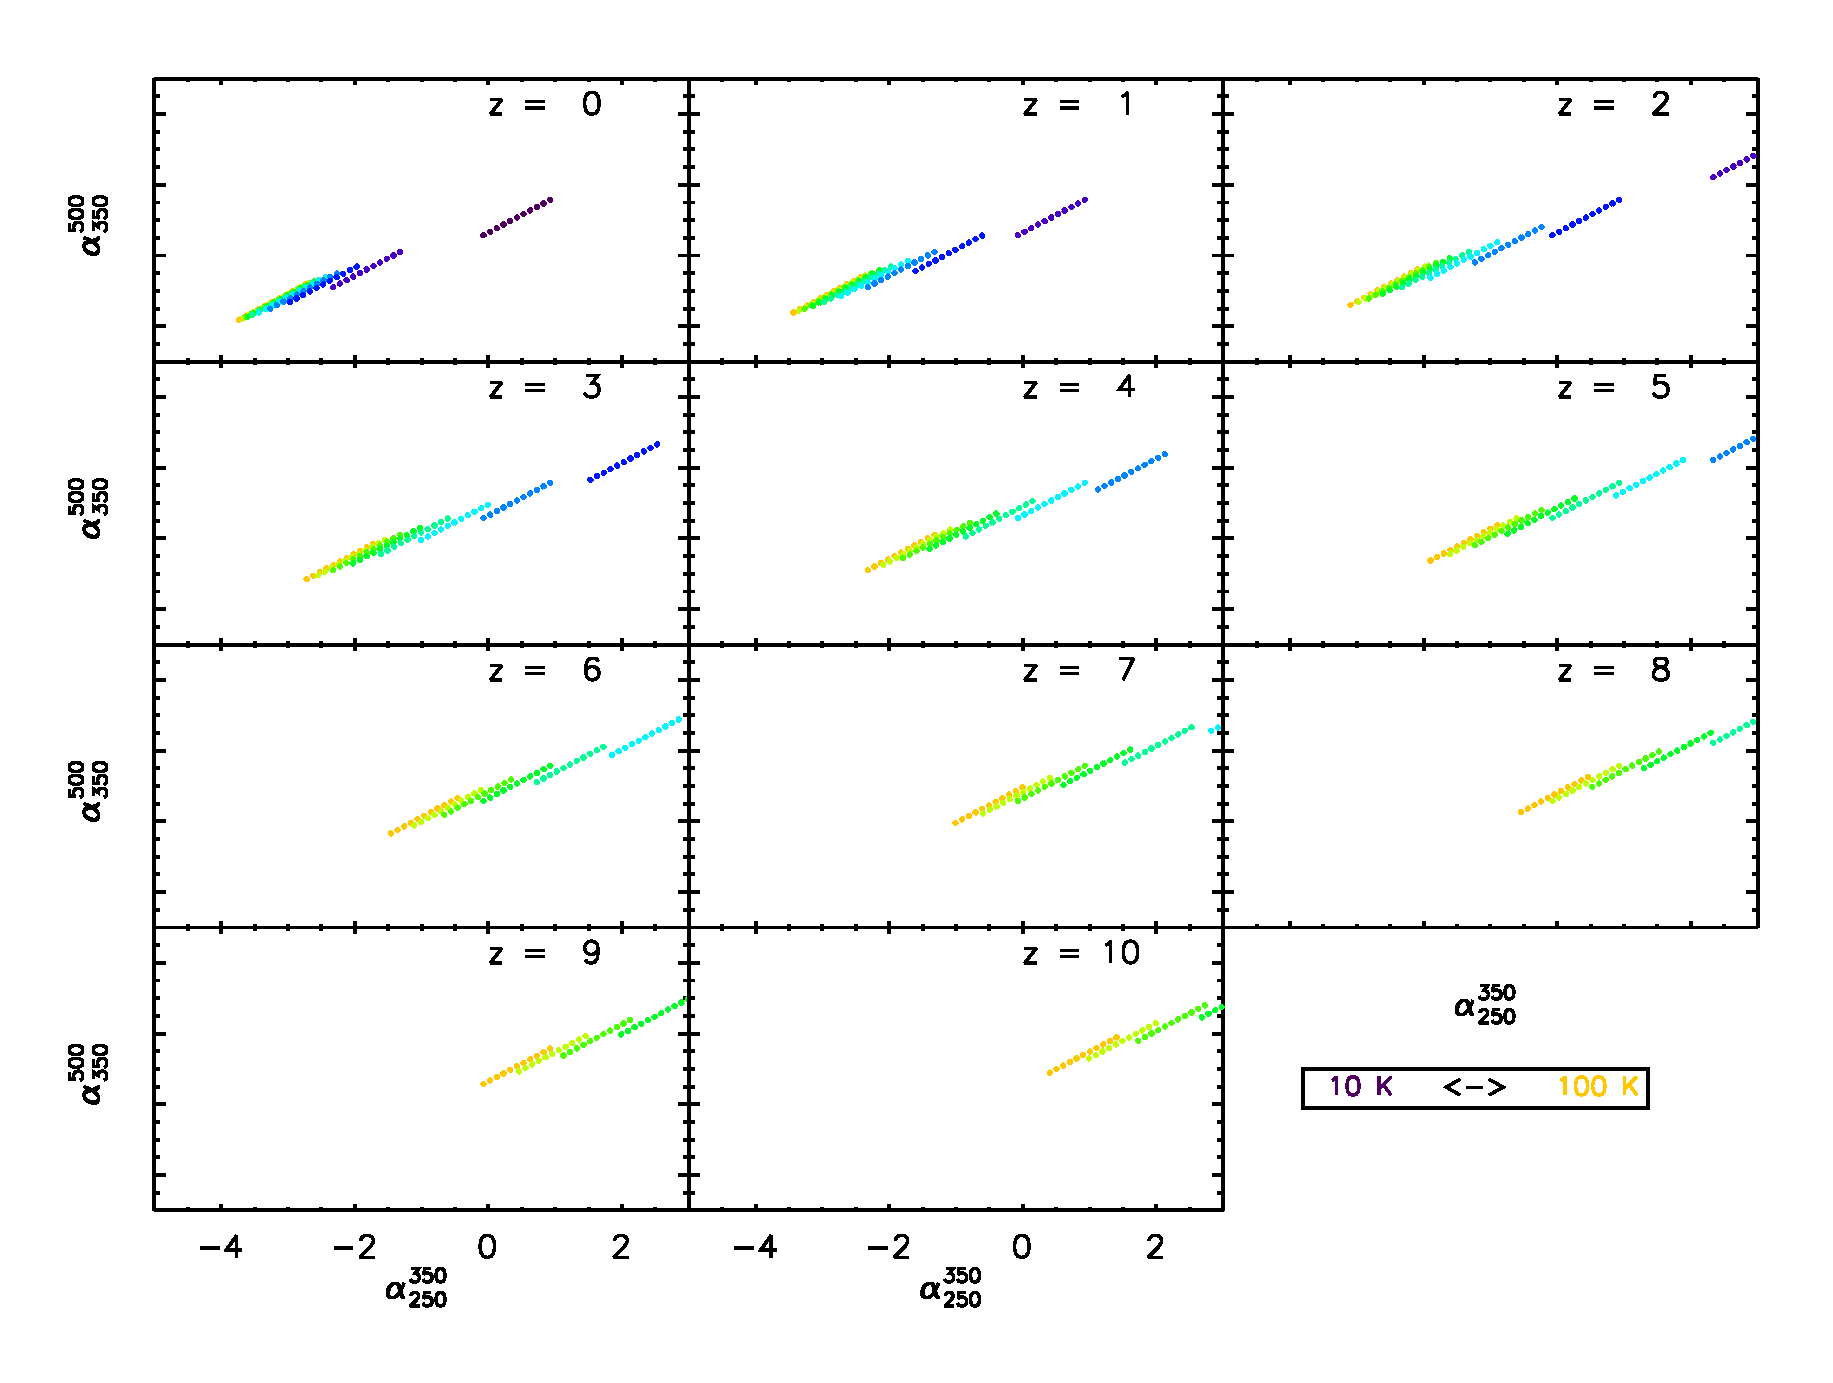
\includegraphics[width=\textwidth]{template_colors.eps}
  \caption{The spectral color pairs produced by the entire library of models for $0<z<10$. It should be noted that the full space of coverage includes all points which lie between any two given points on the above plots, as the model space has effectively infinitely small resolution.}
  \label{slib_color}
\end{figure*}

\begin{figure*}
  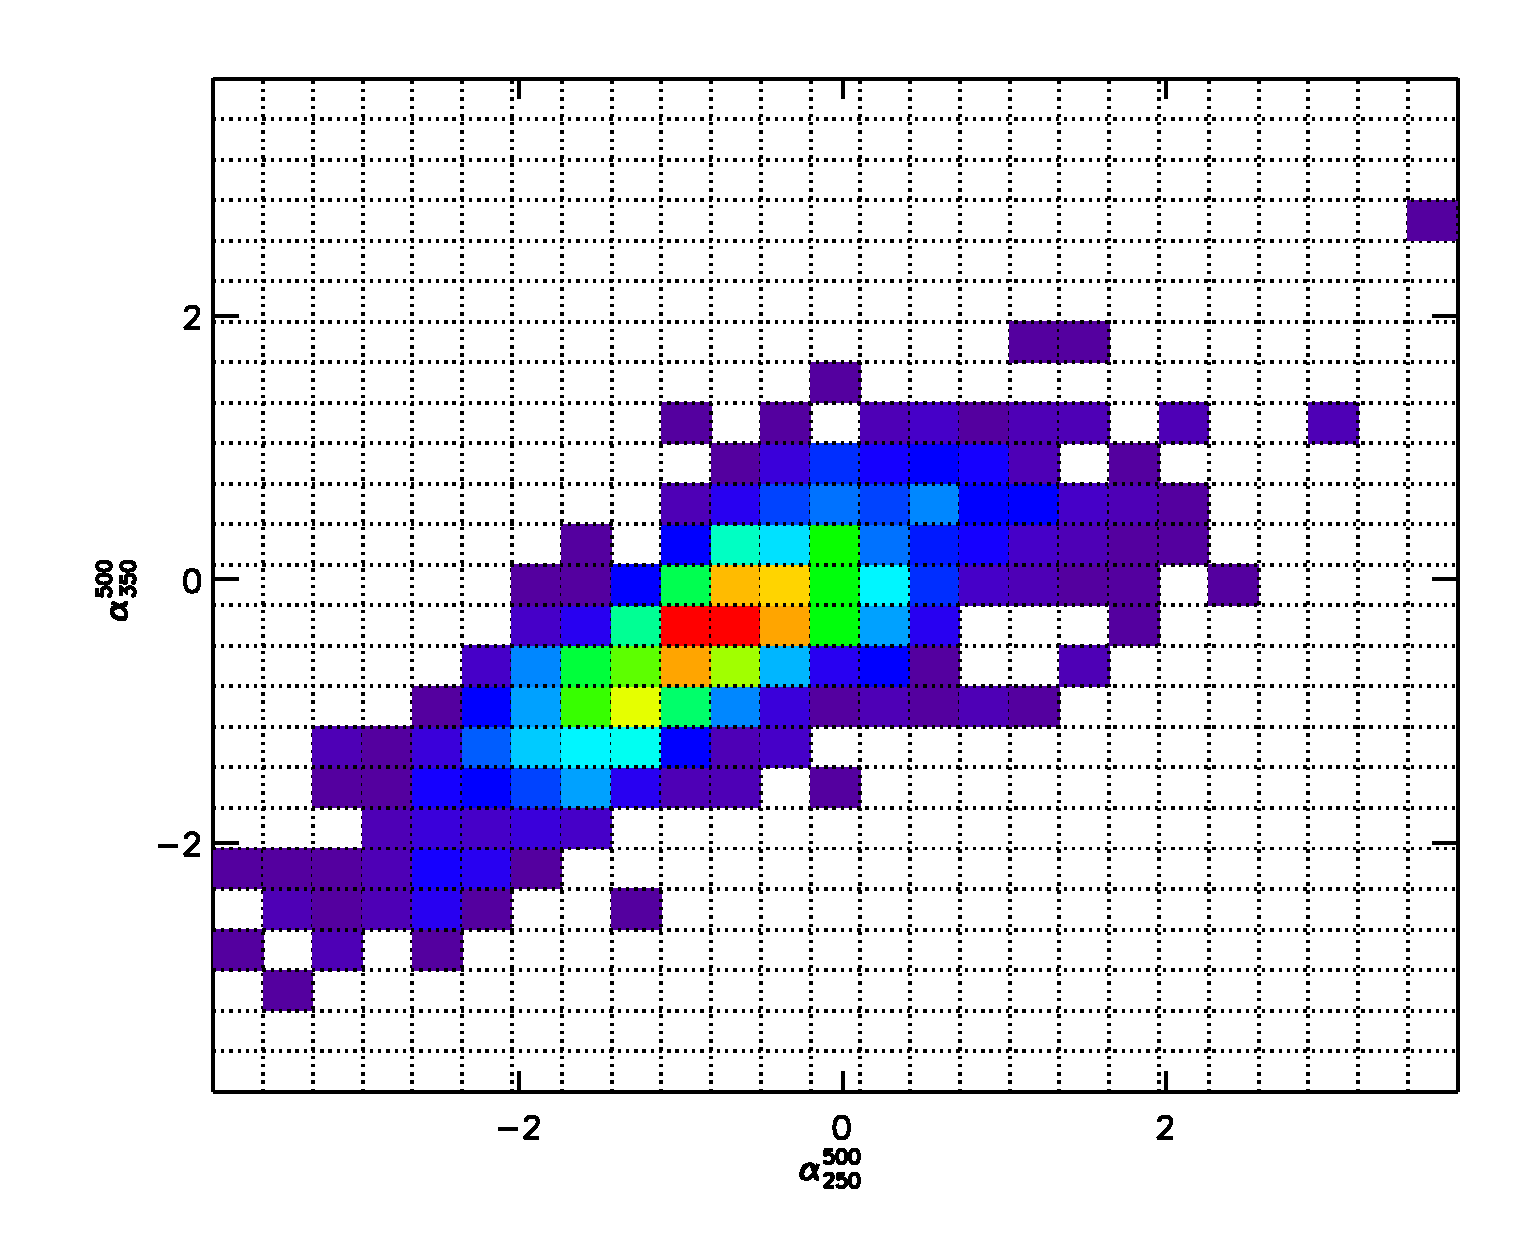
\includegraphics[width=\textwidth]{obs_color_hist.eps}
  \caption{An example of 2-D Color Histogram, created with the HerMES survey data}
  \label{fig:hist1}
\end{figure*}

\begin{figure*}
  \centering
  \includegraphics{fitting2.png}
  \caption{The output from a typical run of the C++ executable. For each run, the best fitting parameters and the goodness-of-fit statistic are output, and if they are at a minimum, the program saves the results to an output fits file. After all fitting passes, the program outputs the best fit parameters of all 10 passes.}
  \label{disp:fit}
\end{figure*}

\begin{figure*}
  \includegraphics[width=\textwidth]{initial.png}
  \caption{The IDL initial fitting window. At the top are the band parameters, below are the redshift and model parameters, and to the right are the luminosity function and cosmological parameters. The run simulation button creates fits files and runs the C++ executable, while the plot last run button reads the output.fits file in the current directory and produces the output seen in Figure \ref{disp:res}.}
  \label{disp:init}
\end{figure*}

\begin{figure*}
  \includegraphics[width=\textwidth]{fitting.png}
  \caption{The IDL results display. The top row of the display (left to right) shows the luminosities of the simulated sources, as well as the fitted redshift distribution and the model parameter distributions used. The second row shows differential source counts, however evolution effects have not been removed, as they will in future version. The final row shows the model, observed, and comparison histograms from the simulation.}
  \label{disp:res}
\end{figure*}

\end{document}
